\section{Marco Teórico}

\subsection{Circuito RLC serie}

Un circuito \textbf{RLC serie} está formado por tres elementos pasivos (es decir, que no pueden generar, amplificar ni controlar de forma activa la energía eléctrica por sí mismos; solo pueden absorberla, almacenarla y liberarla) conectados uno detrás de otro: 

\begin{itemize}
    \item \textbf{R:} Resistencia $R$
    \item \textbf{L:} Inductancia $L$
    \item \textbf{C:} Capacitancia $C$
    \item Una fuente de tensión alterna $v(t)$
\end{itemize}

Dado que están conectados en serie, existe una caracterización fundamental regida por la conservación de la carga, lo que implica que la corriente es la misma en todos los componentes:

\begin{equation}
    i_{R}(t) = i_{L}(t) = i_{C}(t) = i(t)
\end{equation}

Es decir, \textbf{la misma corriente instantánea atraviesa los tres elementos.} Esto es fundamental porque, aunque la corriente sea la misma, el voltaje en cada elemento no está necesariamente en fase con ella \cite{REF_1}.

\begin{figure}[htbp]
    \centering
    \begin{circuitikz}[american, scale=1.2, transform shape]
        % Fuente senoidal a la izquierda, luego R, L, C en serie
        \draw (0,0) to[sinusoidal voltage source, l=$v_s(t)$, invert] (0,3)
              to[short, i=$i(t)$] (1.5,3)
              to[R, l=$R$, v=$v_R$] (4.5,3)
              to[L, l=$L$, v=$v_L$] (7.5,3)
              to[C, l=$C$, v=$v_C$] (7.5,0)
              to[short] (0,0);
    \end{circuitikz}
    \caption{Diagrama esquemático de un circuito RLC en serie.}
    \label{fig:circuit_RLC}
\end{figure}

La fase relativa entre la corriente y la fuerza electromotriz (FEM) no es evidente cuando los tres elementos están presentes. En consecuencia, representamos la corriente mediante la expresión general:

\begin{equation}
    i(t) = I_{0}\sin(\omega t - \phi)
\end{equation}

\begin{figure}[htbp]
    \centering
    \includegraphics[width=0.8\textwidth]{imagenes/CIrcuito_RLC_serie.png}
    \caption{Desfase entre corriente y voltaje en un circuito RLC serie.}
    \label{fig:desfase_rlc}
\end{figure}
Donde $I_0$ es la amplitud de la corriente y $\phi$ es el \textbf{ángulo de fase} entre la corriente y el voltaje aplicado. Por tanto, el ángulo de fase representa la diferencia de fase entre el voltaje y la corriente en el circuito.

Un diagrama fasorial que incluya $i(t)$, $v_R(t)$, $v_C(t)$ y $v_L(t)$ resulta útil para analizar el comportamiento del circuito. Como se muestra en la Figura \ref{fig:diagrama_fasorial_rlc}, el fasor que representa a $v_R(t)$ apunta en la misma dirección que el fasor correspondiente a $i(t)$, y su amplitud está dada por

$$
V_R = I_0R.
$$

El fasor correspondiente a $v_C(t)$ se retrasa $\pi/2$ rad respecto al fasor de $i(t)$ y tiene una amplitud

$$
V_C = I_0X_C.
$$

Por otro lado, el fasor que representa a $v_L(t)$ se adelanta $\pi/2$ rad respecto al fasor de $i(t)$ y presenta una amplitud

$$
V_L = I_0X_L.
$$

\begin{figure}[htbp]
    \centering
    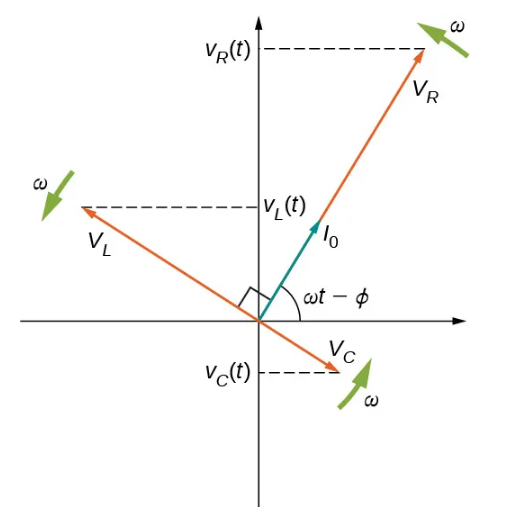
\includegraphics[width=0.7\textwidth]{Imagenes/diagrama_fasorial_rlc.png}
    \caption{Diagrama fasorial de voltajes y corriente en un circuito RLC en serie. 
    Fuente: adaptado de OpenStax, \textit{Física Universitaria Volumen 2}, Sección 15.3.}
    \label{fig:diagrama_fasorial_rlc}
\end{figure}

\subsection{Comportamiento de cada elemento}

Para entender el circuito \textbf{RLC} completo, primero es necesario comprender el comportamiento individual de cada componente.

\subsubsection{Resistencia}

Para una resistencia, la relación fundamental viene dada por la ley de Ohm:
\begin{equation}
    V_{R} = IR
\end{equation}

La tensión y la corriente están en fase. Esto significa que cuando la corriente alcanza su valor máximo, el voltaje también lo hace. Además, la resistencia es el único elemento que \textbf{disipa energía} en forma de calor mediante el efecto Joule:
\begin{equation}
    P_{R} = I_{\text{rms}}^{2}R
\end{equation}

\subsubsection{Inductor}

Un inductor almacena energía en un campo magnético. Su relación tensión-corriente fundamental es:
\begin{equation}
    \boxed{V_{L} = L\frac{di}{dt}}
\end{equation}

Si la corriente alterna se define como:
\begin{equation}
    i(t) = I_{0}\sin(\omega t)
\end{equation}

Entonces el voltaje resulta en:
\begin{equation}
    V_{L} = V_{L0}\sin(\omega t + 90^{\circ})
\end{equation}

Por lo tanto, como se observa en la \ref{fig:diagrama_fasorial_rlc}, en un inductor el voltaje adelanta a la corriente en $90^{\circ}$.

La reactancia inductiva se define como:
\begin{equation}
    X_{L} = 2\pi f L
\end{equation}

De este modo, la reactancia inductiva es directamente proporcional a la frecuencia ($X_{L} \propto f$). Es decir, el inductor ofrece una mayor oposición al paso de la corriente a medida que aumenta la frecuencia de la señal.

\subsubsection{Capacitor}

El capacitor almacena energía en un campo eléctrico. Su ecuación fundamental es:
\begin{equation}
    \boxed{i = C\frac{dV}{dt}}
\end{equation}

En este componente ocurre lo contrario que en el inductor: \textbf{la corriente adelanta al voltaje en $90^{\circ}$}.

La reactancia capacitiva se define como:
\begin{equation}
    X_{C} = \frac{1}{2\pi f C}
\end{equation}

Por lo tanto, la reactancia capacitiva es inversamente proporcional a la frecuencia ($X_{C} \propto \frac{1}{f}$). Esto significa que el condensador ofrece cada vez menos oposición al paso de la corriente a medida que aumenta la frecuencia.

\subsection{Idea Fundamental Circuito RLC}

Podemos definir la reactancia neta: 

\begin{equation}
   \boxed{ 
   X = X_{L} - X_{C}
   }
\end{equation}

Es decir: 

\begin{equation}
    \boxed{
        X = \omega L - \frac{1}{\omega C}
    }
\end{equation}

Donde tenemos tres casos posibles. 

\begin{enumerate}
    \item \textbf{Caso 1:} $X_{L} < X_{C}$ El circuito se comporta predominantemente como capacitivo $X < 0$ la corriente adelanta al voltaje.
    \item \textbf{Caso 2:} $X_{L} > X_{C}$ El circuito se comporta predominantemente como inductivo $X > 0$ la corriente se retrasa respecto al voltaje.
    \item \textbf{Caso 3:} $ X_{L} = X_{C}$ X Condiciones de resonancia $ X = 0$ 
\end{enumerate}

\subsection{Impedancia en un circuito RLC serie}

En un circuito de corriente alterna, la oposición al paso de la corriente no depende únicamente de la resistencia eléctrica, sino también de la presencia de elementos inductivos y capacitivos. Por esta razón, se introduce la impedancia, una magnitud que describe la oposición total que presenta el circuito al paso de la corriente alterna y que tiene en cuenta tanto la amplitud como la diferencia de fase entre la tensión y la corriente.

Para un circuito RLC serie, la magnitud de la impedancia está dada por

\begin{equation}
    \boxed{
        Z = \sqrt{R^2 + \left(\omega L - \frac{1}{\omega C}\right)^2}
    }
    \label{eq:impedancia_rlc}
\end{equation}

donde $R$ es la resistencia total del circuito, $L$ la inductancia, $C$ la capacitancia y $\omega$ la frecuencia angular de la señal aplicada. Las reactancias inductiva y capacitiva se definen, respectivamente, como

\begin{equation}
    X_L = \omega L,
    \qquad
    X_C = \frac{1}{\omega C}.
\end{equation}

Por tanto, la impedancia también puede expresarse como

\begin{equation}
    \boxed{
        Z = \sqrt{R^2 + (X_L-X_C)^2}
    }
\end{equation}

La impedancia no se obtiene mediante la suma directa de la resistencia y las dos reactancias, es decir, $Z \neq R+X_L+X_C$. Esto se debe a que la resistencia y las reactancias representan contribuciones eléctricas con relaciones de fase diferentes. En el análisis fasorial, la resistencia corresponde a la componente real de la impedancia, mientras que la diferencia entre las reactancias inductiva y capacitiva constituye su componente imaginaria. En consecuencia, la magnitud de la impedancia se obtiene mediante la combinación geométrica de ambas componentes.

Aplicando la ley de Ohm en corriente alterna, la corriente eficaz del circuito se relaciona con la tensión eficaz de la fuente mediante

\begin{equation}
    \boxed{
        I_{\mathrm{rms}} = \frac{V_{\mathrm{rms}}}{Z}
    }
    \label{eq:ley_ohm_rlc}
\end{equation}

De esta expresión se deduce que, para una tensión eficaz constante, un aumento de la impedancia produce una disminución de la corriente eficaz. Por el contrario, cuando la impedancia disminuye, la corriente aumenta. Este comportamiento permite comprender por qué la corriente alcanza un valor máximo en la condición de resonancia de un circuito RLC serie ideal.

\subsection{Ángulo de fase y frecuencia de resonancia}

En un circuito RLC serie, la tensión de la fuente y la corriente pueden presentar una diferencia de fase debido a la presencia de la inductancia y la capacitancia. Esta diferencia se describe mediante el ángulo de fase $\phi$, que puede determinarse a partir del diagrama fasorial del circuito, como se muestra en la Figura~\ref{fig:diagrama_fasorial_rlc}. Su relación con los parámetros eléctricos está dada por

\begin{equation}
    \boxed{
        \tan(\phi) = \frac{X_L-X_C}{R}
    }
    \label{eq:angulo_fase_rlc}
\end{equation}

De manera equivalente, el ángulo de fase puede expresarse como

\begin{equation}
    \phi = \arctan\left(\frac{X_L-X_C}{R}\right).
\end{equation}

Cuando $X_L>X_C$, predomina el comportamiento inductivo y la corriente se retrasa respecto a la tensión. En cambio, cuando $X_C>X_L$, predomina el comportamiento capacitivo y la corriente se adelanta respecto a la tensión.

La resonancia eléctrica en un circuito RLC serie ocurre cuando las reactancias inductiva y capacitiva tienen la misma magnitud:

\begin{equation}
    X_L=X_C.
\end{equation}

Al sustituir las expresiones de ambas reactancias, se obtiene

\begin{equation}
    \omega L = \frac{1}{\omega C}.
\end{equation}

Despejando la frecuencia angular, resulta

\begin{equation}
    \boxed{
        \omega_0 = \frac{1}{\sqrt{LC}}
    }
    \label{eq:frecuencia_angular_resonancia}
\end{equation}

Dado que la frecuencia angular se relaciona con la frecuencia mediante $\omega_0=2\pi f_0$, la frecuencia de resonancia teórica está dada por

\begin{equation}
    \boxed{
        f_0 = \frac{1}{2\pi\sqrt{LC}}
    }
    \label{eq:frecuencia_resonancia}
\end{equation}

En la condición de resonancia, las contribuciones inductiva y capacitiva se cancelan en la impedancia. Por consiguiente, para un circuito RLC serie ideal, la impedancia alcanza su valor mínimo, $Z=R$, y el ángulo de fase es nulo, $\phi=0$. En estas condiciones, la tensión de la fuente y la corriente están en fase y, si la tensión eficaz permanece constante, la corriente eficaz alcanza su valor máximo.

\subsection{Intercambio de energía en el circuito RLC}

El comportamiento resonante también puede interpretarse a partir del almacenamiento y la transferencia de energía entre el campo eléctrico del capacitor y el campo magnético del inductor. La energía almacenada en un capacitor de capacitancia $C$, cuando la diferencia de potencial entre sus terminales es $V_C$, está dada por

\begin{equation}
    \boxed{
        U_C = \frac{1}{2}CV_C^2
    }
    \label{eq:energia_capacitor}
\end{equation}

Por su parte, la energía almacenada en un inductor de inductancia $L$, cuando circula una corriente $i_L$, es

\begin{equation}
    \boxed{
        U_L = \frac{1}{2}Li_L^2
    }
    \label{eq:energia_inductor}
\end{equation}

En un circuito LC ideal, la energía puede intercambiarse periódicamente entre el capacitor y el inductor: el capacitor almacena energía en su campo eléctrico y, durante la descarga, la corriente genera un campo magnético en el inductor. Posteriormente, la energía magnética puede contribuir a recargar el capacitor con polaridad opuesta, repitiéndose el proceso.

En un circuito RLC real, parte de la energía se disipa en forma de calor debido a la resistencia eléctrica. Por ello, el intercambio de energía entre los elementos reactivos no es completamente conservativo. Cuando existe una fuente alterna, esta suministra energía al circuito y puede compensar la energía disipada, manteniendo las oscilaciones eléctricas. La respuesta del circuito depende de la frecuencia de excitación y alcanza su condición de resonancia cuando se igualan las magnitudes de las reactancias inductiva y capacitiva.

\subsection{Analogía mecánica del circuito RLC}

El comportamiento de un circuito RLC serie puede compararse con el de un sistema mecánico formado por una masa, un resorte y un amortiguador. Esta analogía permite interpretar la resonancia eléctrica mediante conceptos conocidos de oscilaciones mecánicas.

\begin{table}[htbp]
    \centering
    \caption{Analogía entre un circuito RLC serie y un sistema masa-resorte-amortiguador.}
    \label{tab:analogia_mecanica}
    \begin{tabular}{|l|l|}
        \hline
        \textbf{Sistema mecánico} & \textbf{Circuito RLC serie} \\ \hline
        Masa $m$ & Inductancia $L$ \\ \hline
        Constante elástica $k$ & Inverso de la capacitancia $1/C$ \\ \hline
        Amortiguamiento viscoso $b$ & Resistencia $R$ \\ \hline
        Fuerza externa & Tensión de la fuente $V(t)$ \\ \hline
        Velocidad $v(t)$ & Corriente $i(t)$ \\ \hline
        Desplazamiento $x(t)$ & Carga eléctrica $q(t)$ \\ \hline
        Frecuencia natural $\sqrt{k/m}$ & Frecuencia angular $1/\sqrt{LC}$ \\ \hline
    \end{tabular}
\end{table}

En esta correspondencia, la inductancia representa la inercia del sistema, ya que se opone a los cambios de corriente, mientras que el capacitor se comporta de manera análoga al resorte, pues su tensión depende de la carga almacenada. La resistencia representa el amortiguamiento mecánico, dado que disipa energía y limita la amplitud de la respuesta. Finalmente, la fuente de tensión desempeña un papel análogo al de una fuerza externa que excita el sistema.

\begin{figure}[htbp]
    \centering
    \includegraphics[width=0.75\textwidth]{imagenes/diagrama_masa_resorte.png}
    \caption{Representación esquemática de un sistema mecánico masa-resorte-amortiguador.}
    \label{fig:masa_resorte}
\end{figure}

\subsection{Factor de calidad}

El factor de calidad \(Q\) es un parámetro adimensional que permite caracterizar la selectividad de un circuito resonante y cuantificar la relación entre la energía almacenada y la energía disipada durante su funcionamiento. De acuerdo con la interpretación energética, se define como la razón entre la energía total almacenada en el sistema y la energía perdida por ciclo, multiplicada por \(2\pi\):

\begin{equation}
    Q = 2\pi \frac{E}{\Delta E},
    \label{eq:Q_energia}
\end{equation}

donde \(E\) representa la energía almacenada y \(\Delta E\) corresponde a la energía disipada durante un ciclo. En un circuito RLC serie, la resistencia es responsable de las pérdidas de energía por efecto Joule, mientras que el inductor y el capacitor permiten almacenar e intercambiar energía mediante sus campos magnético y eléctrico, respectivamente \cite{REF_2}.

Para un circuito RLC serie idealizado, alimentado por una fuente sinusoidal, el factor de calidad puede expresarse en función de la frecuencia angular de resonancia \(\omega_0\), la inductancia \(L\) y la resistencia total \(R\) como

\begin{equation}
    Q = \frac{\omega_0 L}{R}.
    \label{eq:Q_RLC}
\end{equation}

Puesto que la frecuencia angular de resonancia está relacionada con la inductancia y la capacitancia mediante

\begin{equation}
    \omega_0 = \frac{1}{\sqrt{LC}},
    \label{eq:omega_res_Q}
\end{equation}

el factor de calidad también puede escribirse como

\begin{equation}
    Q = \frac{1}{R}\sqrt{\frac{L}{C}}.
    \label{eq:Q_LC}
\end{equation}

En estas expresiones, \(R\) corresponde a la resistencia total efectiva del circuito, incluyendo las contribuciones resistivas relevantes de sus componentes y de la fuente. Por tanto, no debe confundirse necesariamente con la resistencia externa conectada durante el experimento.

Físicamente, un valor elevado de \(Q\) indica que las pérdidas de energía son relativamente pequeñas y que la respuesta del circuito está concentrada en un intervalo estrecho de frecuencias alrededor de la resonancia. Por el contrario, un valor reducido de \(Q\) corresponde a una respuesta resonante más amplia y menos selectiva. De acuerdo con la ecuación \eqref{eq:Q_RLC}, para valores constantes de \(L\) y \(C\), el factor de calidad disminuye al aumentar la resistencia total del circuito.

El factor de calidad también puede relacionarse con el ancho de banda de la respuesta resonante. Si \(f_0\) es la frecuencia de resonancia y \(f_L\) y \(f_H\) son, respectivamente, las frecuencias inferior y superior de media potencia, el ancho de banda se define como

\begin{equation}
    \Delta f_{\mathrm{BW}} = f_H-f_L.
    \label{eq:ancho_banda}
\end{equation}

Para un circuito RLC serie idealizado, el ancho de banda expresado en hertz está dado por

\begin{equation}
    \Delta f_{\mathrm{BW}} = \frac{R}{2\pi L}.
    \label{eq:BW_RLC}
\end{equation}

En consecuencia, el factor de calidad puede expresarse como la razón entre la frecuencia de resonancia y el ancho de banda:

\begin{equation}
    Q = \frac{f_0}{\Delta f_{\mathrm{BW}}}.
    \label{eq:Q_BW}
\end{equation}

Las frecuencias \(f_L\) y \(f_H\) corresponden a los puntos en los cuales la potencia disipada en la resistencia es la mitad de su valor máximo. Debido a que la potencia es proporcional al cuadrado de la corriente eficaz, en dichos puntos se cumple

\begin{equation}
    I_{\mathrm{rms}} = \frac{I_{\mathrm{rms,max}}}{\sqrt{2}}.
    \label{eq:media_potencia}
\end{equation}

Esta relación permite determinar experimentalmente el ancho de banda a partir de la curva de corriente eficaz en función de la frecuencia. En particular, un circuito con mayor factor de calidad presenta una curva de resonancia más estrecha, mientras que un circuito con menor factor de calidad presenta una curva más ancha.

En la práctica del circuito RLC serie resonante, la comparación de las curvas obtenidas para diferentes valores de resistencia permite estudiar experimentalmente esta dependencia. Al aumentar la resistencia total, la corriente máxima disminuye y el ancho de banda aumenta, de acuerdo con las ecuaciones \eqref{eq:Q_RLC} y \eqref{eq:BW_RLC}. Por tanto, el factor de calidad constituye una magnitud útil para relacionar las pérdidas resistivas del circuito con la selectividad de su respuesta en frecuencia \cite{REF_2}.

































